\documentclass[12pt]{article} % 12pt 为字号大小 UTF8
\usepackage{amssymb,amsfonts,amsmath,amsthm}
%\usepackage{fontspec,xltxtra,xunicode}
%\usepackage{times}

%----------
% 定义中文环境
%----------

\usepackage{xeCJK}

% \setCJKmainfont[BoldFont={SimHei},ItalicFont={KaiTi}]{SimSun}
% \setCJKsansfont{SimHei}
% \setCJKfamilyfont{zhsong}{SimSun}
% \setCJKfamilyfont{zhhei}{SimHei}

% \newcommand*{\songti}{\CJKfamily{zhsong}} % 宋体
% \newcommand*{\heiti}{\CJKfamily{zhhei}}   % 黑体


%----------
% 版面设置
%----------
%首段缩进
\usepackage{indentfirst}
\setlength{\parindent}{2.1em}

%行距
\renewcommand{\baselinestretch}{1.2} % 1.4倍行距

%页边距
\usepackage[a4paper]{geometry}
\geometry{verbose,
  tmargin=3cm,% 上边距
  bmargin=3cm,% 下边距
  lmargin=3cm,% 左边距
  rmargin=3cm % 右边距
}


%----------
% 其他宏包
%----------
%图形相关
\usepackage[x11names]{xcolor} % must before tikz, x11names defines RoyalBlue3
\usepackage{graphicx}
\usepackage{pstricks,pst-plot,pst-eps}
\usepackage{subfig}
\def\pgfsysdriver{pgfsys-dvipdfmx.def} % put before tikz
\usepackage{tikz}

%原文照排
\usepackage{verbatim}
\usepackage{float}

%网址
\usepackage{url}

%文本格式
\usepackage{ulem} % 用法:\uline{}下划线,\uwave{}波浪线,\sout{}删除线
\usepackage{pifont} % 用法:\ding{数字}代表数字被圈起来
\usepackage{enumitem} % 使用enumitem宏包自定义列表样式
\usepackage{hyperref} % 不仅可以帮助你插入链接,还能让这些链接在生成的PDF文档中是可点击的,提高文档的互动性,用法:\url{http://www.example.com}


%----------
% 习题与解答环境
%----------
%习题环境
\theoremstyle{definition} 
\newtheorem{problem}{题目}

%解答环境
\ifx\proof\undefined\
\newenvironment{proof}[1][\protect\proofname]{\par
\normalfont\topsep6\p@\@plus6\p@\relax
\trivlist
\itemindent\parindent
\item[\hskip\labelsep
\scshape
#1]\ignorespaces
}{%
\endtrivlist\@endpefalse
}
\fi
\renewcommand{\proofname}{\it{解答}}


%----------
% 我的自定义
%----------

\newcommand{\horrule}[1]{\rule[0.5ex]{\linewidth}{#1}} 	% Horizontal rule

\renewcommand{\refname}{参考文献}
\renewcommand{\abstractname}{\large \bf 摘\quad 要}
\renewcommand{\contentsname}{目录}
\renewcommand{\tablename}{表}
\renewcommand{\figurename}{图}

\setlength{\parskip}{0.4ex} % 段落间距

\usepackage{enumitem}
\setenumerate[1]{itemsep=0pt,partopsep=0pt,parsep=\parskip,topsep=5pt}
\setitemize[1]{itemsep=0.4ex,partopsep=0.4ex,parsep=\parskip,topsep=0.4ex}
\setdescription{itemsep=0pt,partopsep=0pt,parsep=\parskip,topsep=5pt}


%==========
% 正文部分
%==========

\begin{document}

\title{
{\normalfont\normalsize\textsc{
Peking University\\
Introduction to Database Systems, Spring 2024 \\[25pt]}}
\horrule{0.5pt}\\
\sffamily{第三章\ 关系代数\\课后作业}
\horrule{1.8pt}\\[20pt]
}
\author{梁昱桐\quad 2100013116\\lyt0112@outlook.com}
% \date{} % 若不需要自动插入日期,则去掉前面的注释;{ } 中也可以自定义日期格式

\begin{titlepage}
\maketitle
\vspace{30pt}

% \begin{abstract}
% \normalsize \ \ 这是中文摘要。大概写满这一页可以了。摘要又称概要、内容提要。摘要是以提供文献内容梗概为目的,不加评论和补充解释,简明、确切地记述文献重要内容的短文。其基本要素包括研究目的、方法、结果和结论。具体地讲就是研究工作的主要对象和范围,采用的手段和方法,得出的结果和重要的结论,有时也包括具有情报价值的其它重要的信息。\\[5pt]
% \indent \ \ \textbf{关键词}:图卷积神经网络,复杂网络,表示学习
% \end{abstract}

\thispagestyle{empty}
\end{titlepage}

% \tableofcontents
% \thispagestyle{empty}

\newpage
\setcounter{page}{1}

\begin{problem}
S (SNO, SNAME, CITY)

P (PNO, PNAME, COLOR, PRICE)

J (JNO, JNAME,CITY)

SPJ (SNO, PNO, JNO, QTY)

S表示供应商,各属性依次为供应商号,供应商名,供应商所在城市

P表示零件,各属性依次为零件号,零件名,零件颜色,零件价格

J表示工程,各属性依次为工程号,工程名,工程所在城市

SPJ表示供货关系,各属性依次为供应商号,零件号,工程号,供货数量。

\begin{enumerate}
  \item 求同时向位于北京和天津的工程供应了零件的供应商的供应商名
  \item 求向和自己位于相同城市的工程供应零件的供应商的供应商号
  \item 求只向和自己位于不同城市的工程供应零件的供应商的供应商号
  \item 求向所有位于北京的工程都供应了零件的供应商的供应商号
  \item 求价格最高的零件的零件号
\end{enumerate}

\end{problem}

\begin{proof}

\end{proof}

\begin{problem}
对于选课表SC (sno, cno, grade),完成如下查询:

\begin{enumerate}
  \item 求至少选修了c1和c2课程的学生
  \item 求恰好选修了c1和c2课程的学生(*)
  \item 求选修了所有s1同学所修课程的学生
  \item 求其选修课程被s1同学所修课程完全包含的学生(参考下页)
  \item 求和s1同学所修课程完全不同的学生
  \item 求和s1同学所修课程完全相同的学生(*)
  \item (终极挑战)求所修课程完全相同的学生对(*)
\end{enumerate}

(注意:标*的可以不用做)

\begin{figure}[H]
  \centering
  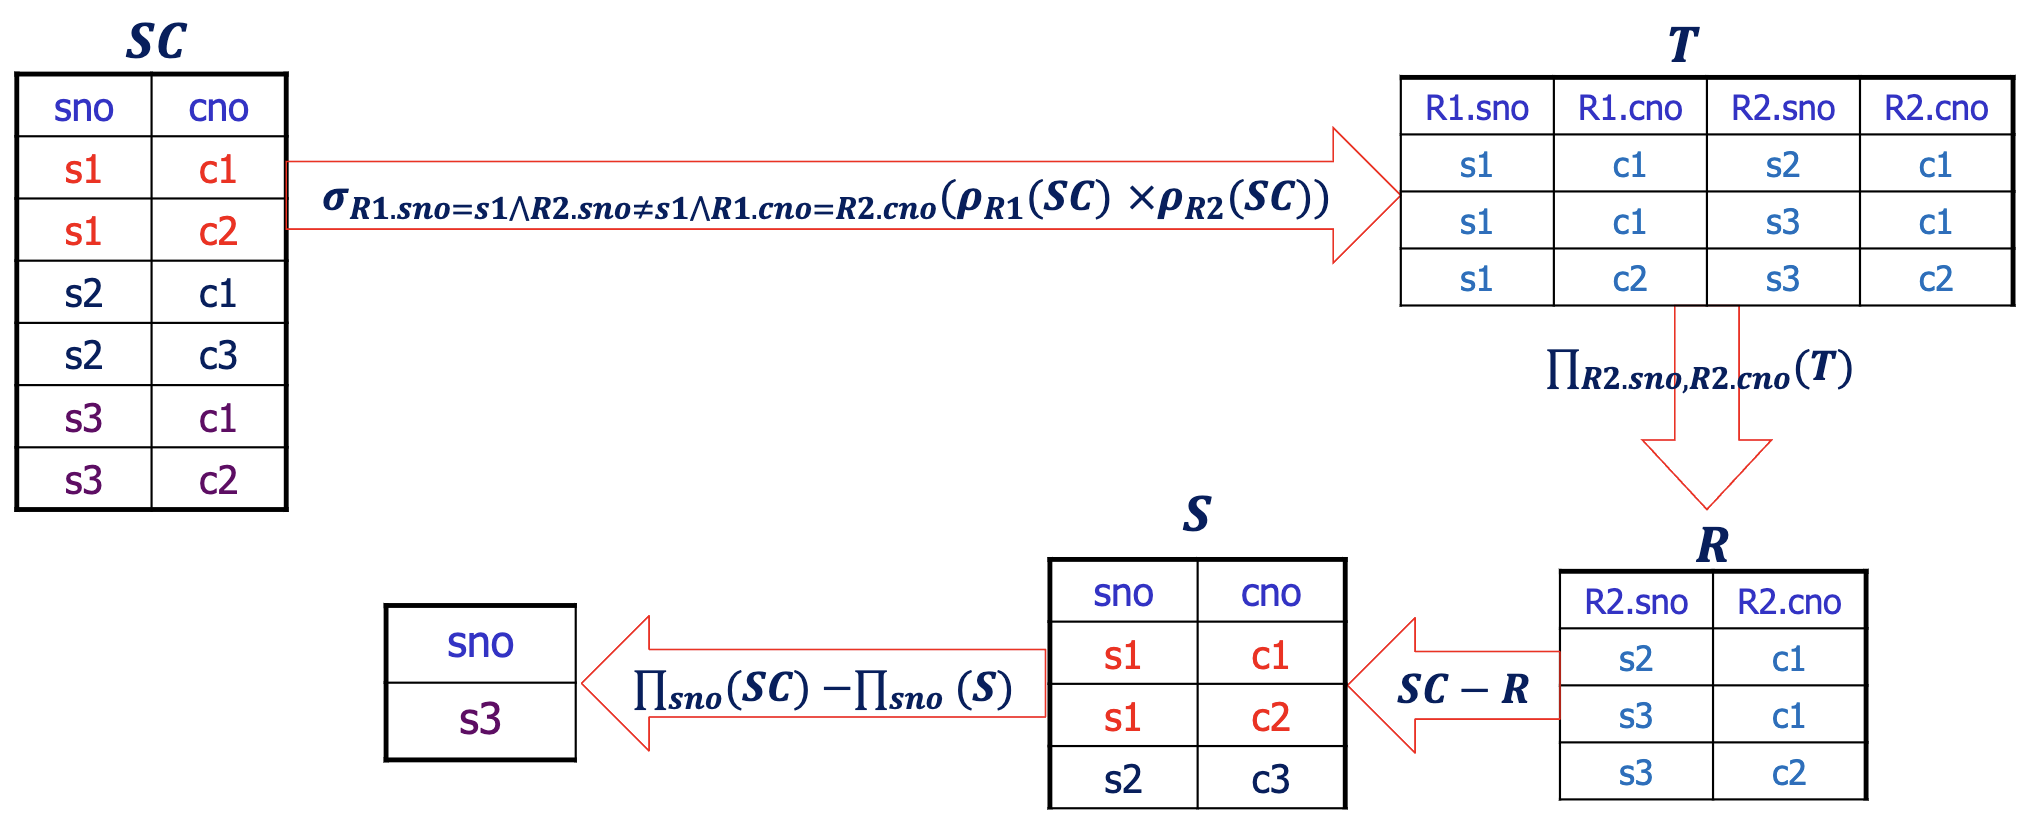
\includegraphics[width=0.8\textwidth]{./figs/2.1.png}
  \caption{示例:求其选修课程被s01号学生所修课程包含的学生号}
\end{figure}

\end{problem}  

\begin{proof}

\end{proof}

\begin{problem}
对于关系R(A, B),用关系代数来检验A是否取值唯一。
更进一步,对于关系R(A, B, C),用关系代数来检验A是否取值唯一。
(注意,“唯一”的意思是两两不同,而不是只取同一个值,那个应该叫“单一”)  
\end{problem}

\begin{proof}

\end{proof}

\begin{problem}
对于选课表SC(sno, cno, grade),分别用元组关系演算和域关系演算,完成如下查询:

\begin{enumerate}
  \item 求同时选修了c1和c2课程的学生
  \item 求选修c1课程成绩比s1同学的该门课程成绩高的学生
\end{enumerate}  
  
\end{problem}

\begin{proof}

\end{proof}

\newpage
\bibliographystyle{plain}
\bibliography{ref}


\end{document}
